
\cp{http://ru.wikibooks.org/wiki/KiCad}

KiCad\ --- распространяемый по лицензии GNU GPL программный комплекс САПР EDA с
открытыми исходными текстами, предназначенный для разработки электрических схем
и печатных плат.

Кроссплатформенность компонентов KiCad обеспечивается использованием 
библиотеки wxWidgets. Поддерживаются операционные системы Linux, 
Windows NT 5.x, Free\-BSD и Solaris.

Разработчик\ --- Жан-Пьер Шарра (фр. Jean-Pierre Charras), исследователь 
в LIS (фр. Laboratoire des Images et des Signaux — Лаборатория Изображений 
и Сигналов) и преподаватель электроники и обработки изображений в фр. 
IUT de Saint Martin d’Hères (Франция).

\bigskip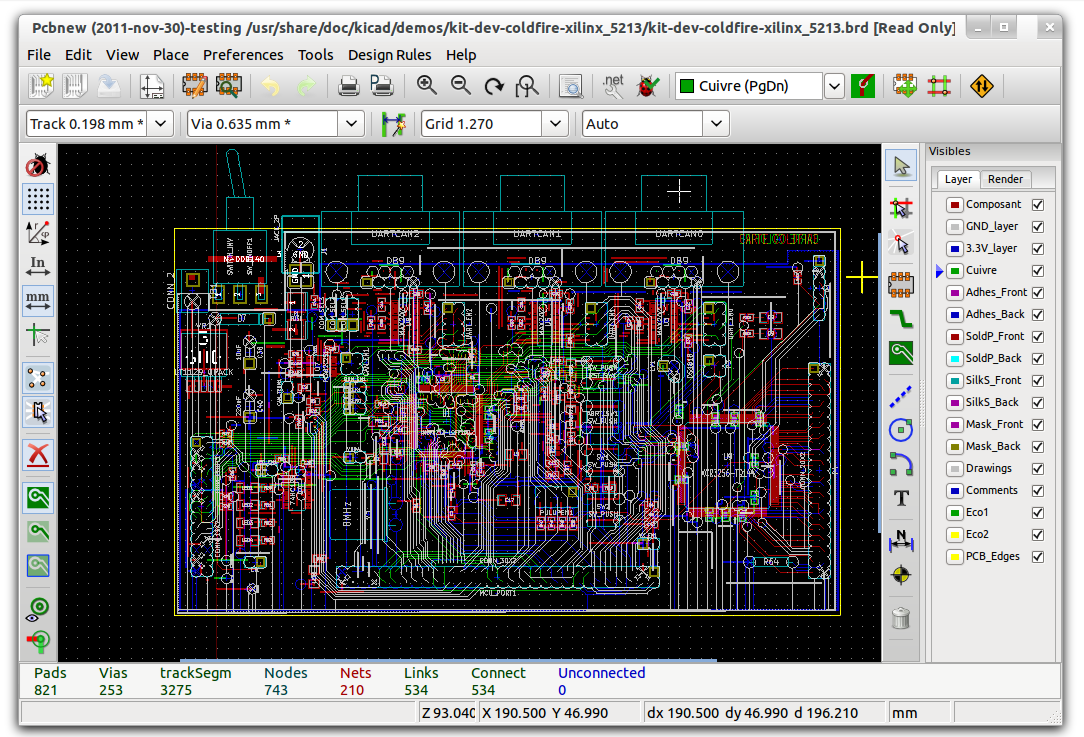
\includegraphics[height=0.5\textheight]{kicad/kicad_pcbnew.png}

